\section{Wstęp teoretyczny}
\subsection{Klasyfikacja sceny}
\begin{figure}
    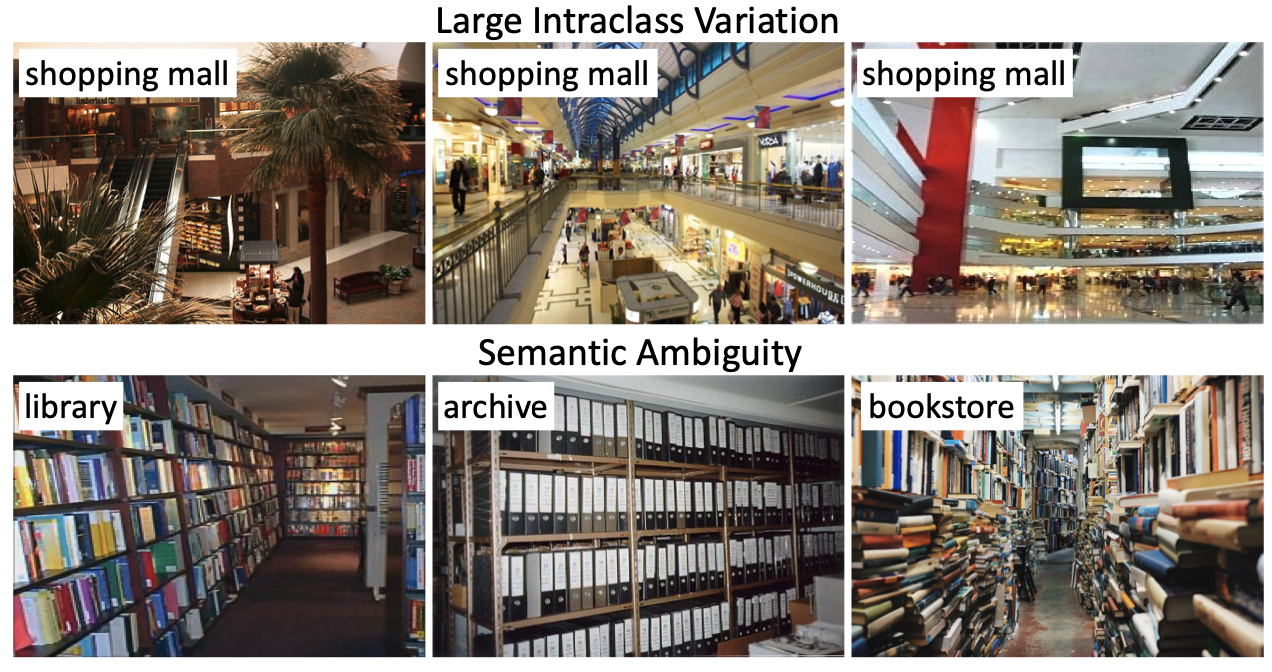
\includegraphics[width=\textwidth]{images/scene_class.png}
    \caption{Problem różrnorodności wewnątrzklasowej oraz wieloznaczności semantycznej \cite{zeng2021deep}.}
    \label{fig:scene-class}
\end{figure}

Zadanie klasyfikacji sceny polega na przyporządkowaniu kategorii miejsca w które przedstawia obraz. Istnieje duża różnica między klasyfikacja obrazka, a klasyfikacją sceny. Klasyfikacja obrazka jako taka zajmuje się przypodrządkowaniem klasy obiektu pierwszoplanowego, np. czy na obrazie znajduje się pies czy kot. Klasyfikacja sceny natomiast musi wziać pod uwagę wszytskie cechy obrazu, zarówno tła jak i pierwszego planu by określić odpowiednie miejsce.

Zadanie klasyfikacji sceny jest trudne ze względu na problem różrnorodności wewnątrzklasowej oraz wieloznaczności semantycznej, co zostało przedstawione na rys. \ref{fig:scene-class}. Pierwszy z nich polega na fakcie, iż jedno miejsce moze zostać przedstawione w bardzo różnej konfiguracji m.in. oświetlenia, ekspozycji, obiektów zajdujących się na obrazie. Drugi jest związany z występowaniem tych samych obiektów dla różnych klas scen.

\subsection{Segmentacja obrazu}
\begin{figure}
    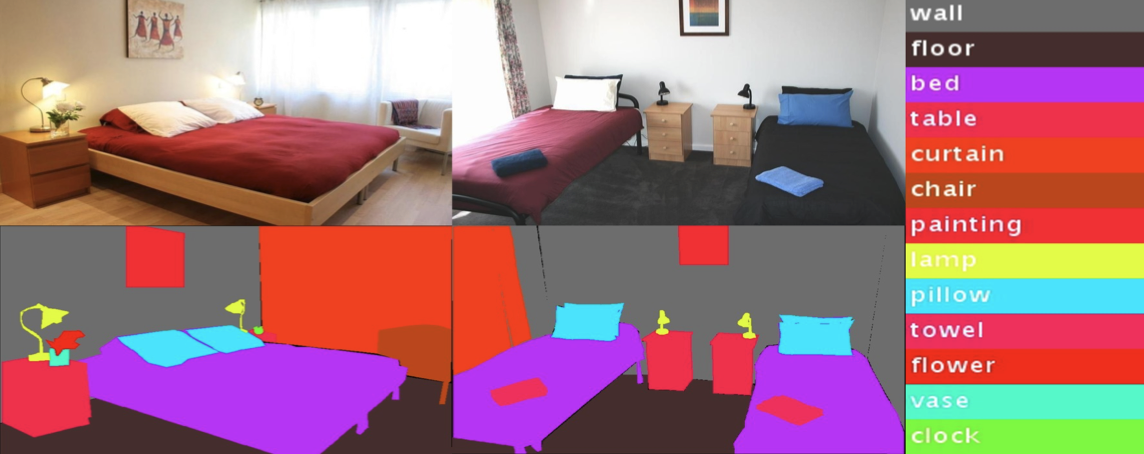
\includegraphics[width=\textwidth]{images/segment.png}
    \caption{Segmentacja wewntątrz pomieszczeń \cite{zhang2018context}.}
    \label{fig:segment}
  \end{figure}

Zadanie segmentacji obrazu to przyporządkowanie każdemu pikselowi etykiety (rys. \ref{fig:segment}). W rezultacie obraz zostaje podzielony na homogeniczne regiony pod względem pewnych własności.

\section{Cel pracy}
Celem pracy inżynierskiej są dwa zadania:
\begin{itemize}
    \item segmentacja środowiska wewntątrz budynku
    \item klasyfikacja pomieszczeń
\end{itemize}
\section{Założenia}
Praca zakłada wykonanie celów pracy w środowisku wewntątrz budynków, co więcej będzie to środowisko domowe. Pondato inferencja zostanie przeporwadzona na robocie Tiago, który jest wyposażony w kamerę Kinect.
\section{Motywacje}
Istnieje wiele powodów dla których temat pracy jest warty uwagi.

Po pierwsze rozwiązanie moze być wykorzystane w nawigacji robota. Wykrywanie przeszkód jest kluczowym aspektem możliwosci poruszania się robota. Zostanie ono podjęte przez zadanie segmentacji. Należy zwrócić uwagę, że robot powinien zachowywać sie ostrożniej w kuchni oraz w łazience. Ta informacja zostanie uzyskana poprzez klasyfikację sceny.

Innym zastosowanie rozważanego rozwiązania jest pomoc dla osób niewidomych. Osoba niepełnosprawa mogłaby wówczas poruszać się po środowisku domowym z większą łatwością, mając na sobie kamerę oraz informaję o otaczajacej przestrzeni.

\section{Zbiór danych}

Zbiór danych powinien ściśle odpowiadać założenią postawionym w pracy. Inferencja wymaga użycia kamery Kinect. Zatem zbiór danych powiniem zawierać kategorie scen, segmentacje obrazow oraz najlepiej byc ujętym przr kamerę Kinect wersji pierwszej.

Po prześledzeniu wielu zbiorów danych udało sie sprostać powyzszym wymaganiom, uzyskując dwa podobne zbiory danych.

\begin{table}[]
    \begin{adjustbox}{width=\columnwidth,center}
    \begin{tabular}{l|ccccccc}
    Nazwa    & \# Ilość & \# Klas obiektów & \# Klas scen & RGB-D     & Rozdzielczość & \# Czujników & Nieposprzątane \\ \hline \hline
    NYUv2    & 1 449    & 894              & 26           & \checkmark & 640 x 480     & 1            & \checkmark                   \\
    SUN RGBD & 10 335   & 800              & 47           & \checkmark & 640 x 480     & 4            & x                         
    \end{tabular}
    \end{adjustbox}
    \caption{Porówanie zbiorów danych \cite{song2015sun},\cite{silberman2012indoor}}
    \label{tab:dataset}
\end{table}

Porównanie zbiorów \texttt{NYUv2} oraz \texttt{SUN RGBD} przedstawiono w tabeli \ref{tab:dataset}. Mimo liczbowej przewagi \texttt{SUN RGBD} pod wieloma względami, ostatecznie wybrano \texttt{NYUv2} z uwagi, że zbiór ten został zebrany dla pomieszczeń, w które nie są posprzątane. Fakt ten uznano, za kluczowy, iż uważano, że będzie przekładał się na lepsze rezultaty w naturalnych warunkach. \texttt{NYUv2} jest też chętniej cytowany niż texttt{SUN RGBD} (rys. \ref{fig:sun-vs-nyu}).

\begin{figure}
    \centering
    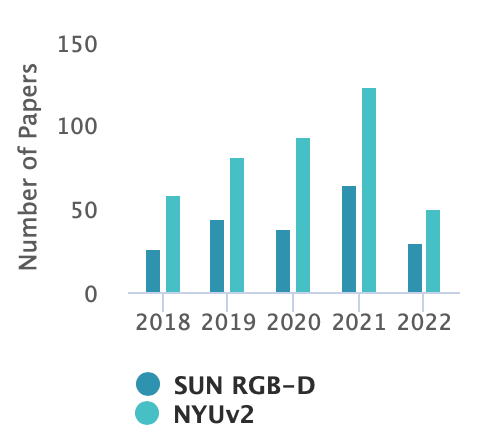
\includegraphics[width=0.5\textwidth]{images/stats-dataset.png}
    \caption[]{Szacowana liczba cytowań w latach 2018-2022 \href{https://paperswithcode.com/dataset/sun-rgb-d}{[paperswithcode.com]}}
    \label{fig:sun-vs-nyu}
\end{figure}

\section{Przegląd rozwiązań}
\subsection{Metody klasyczne}
\begin{figure}
    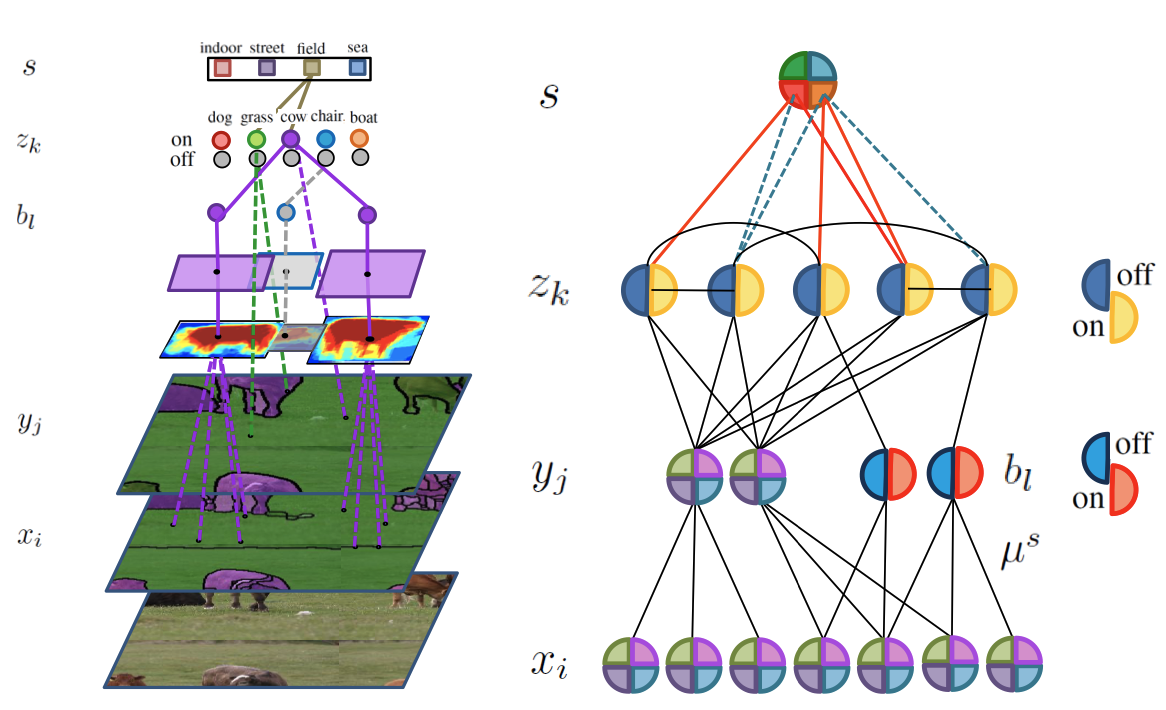
\includegraphics[width=\textwidth]{images/joint-segmentation-and-classification.png}
    \caption{Describing the Scene as a Whole: Joint Object Detection, Scene Classification and Semantic Segmentation 2012 \cite{yao2012describing}.}
    \label{fig:old-school-arch}
\end{figure}